\chapter{Luminometer Calibration}
\label{ch3}

\section{Van Der Meer Method}

The Van Der Meer (vdM) scan let us obtain the value of $\sigma_{visible}$ using different luminometers. For this case the detector of interest is the pixel detector with which are going to obtain a calibration of the luminosity using the vdM scan in combination with the PCC method. The scan consist on separating particle the beams from each other between the X and Y axis by $\Delta X$ and $\Delta Y$ values moving them and recording values of luminosity independently, when the scan on X and scan on Y are imposed over each other we said that they're on head on giving the maximum value of luminosity. Usually a single gaussian fit is used to obtain beam overlap widths also denoted as $\Sigma_{x}$ and $\Sigma_{y}$, other fit models may be used like the doble gaussian depending on the quality of the fit \cite{Vdm}

\begin{figure}[h]
    \centering
    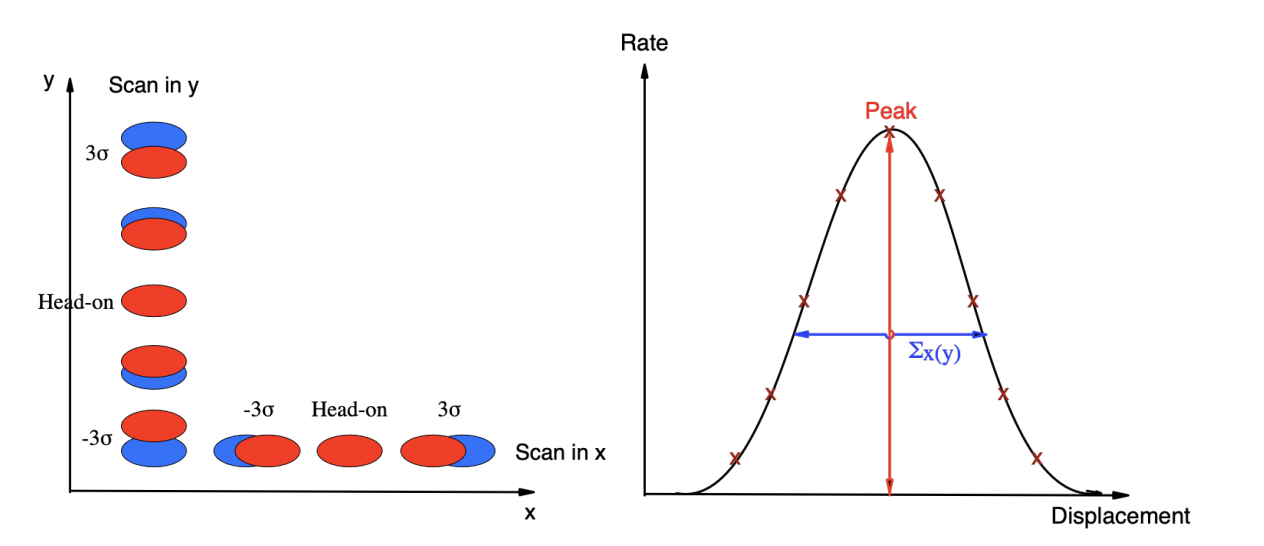
\includegraphics[width=1\textwidth]{vdm1.png}
    \caption{The vdm scan on the left showing the beams for X and Y. On the right a curve of the different values of rate for the beams displacement, the peak occurs during the head on part.}
    \label{fig:vdm1}
\end{figure}


For obtaining the importnat parameters on the vdm scan we return to the equation (1.2) and apply it to and individual bunch crossing, the values of N1 and N2 being the number of protons colliding can be obtained since is a known quantity from the experiment, the frequency f is also a known quantity, the frequency of the LHC which is 11,245 kHz but the proton densities $\rho_{1}$ and $\rho{2}$ are more difficult to obtain, this is were the vdM scan help us to measure integral over the bunch proton densities. The luminosity integral evaluated with the beams separated by a distance $\Delta_{x}$ and $\Delta_{y}$ can take the form of: 

\begin{equation}
 L(\Delta x, \Delta Y) = N_{1} N_{2} f  \int \int \rho_{1}(x,y)\rho_{2}(x+\Delta x, y+\Delta y) dxdy 
\end{equation}

Because of the scan method is it assumed that the two bunches of proton densities are factorizable since they act independently between each other so we can turn the right part of (3.1) into two integrals:

 \begin{equation}
N_{1} N_{2} f  \int \int \rho_{1}(x,y)\rho_{2}(x+\Delta x, y+\Delta y) dxdy   = N_{1} N_{2} f (\int \rho_{1}(x)\rho_{2}(x + \Delta x) dx) (\int rho_{1}(y) \rho_{2}(y + \Delta y) dy)
\end{equation}

Integrating both sides on $\Delta y$ and using in combination with (3.1) while we fix $\Delta x_{0}$ = 0 and $\Delta y_{0}$ = 0 as the head on point,  we obtain:
 
 \begin{equation}
N_{1} N_{2} f \int \rho_{1}(x) \rho_{2}(x + \Delta x_{0}) dx = \int L (\Delta x_{0}, d\Delta y) d(\Delta y)
\end{equation}

A similar result is obtained when we integrate both sides for $\Delta x$ using this and combining equation (3.1), (3.2) and (3.3) we can obtain that 

\begin{equation}
N_{1} N_{2} f \int \rho_{1}(x) \rho_{2}(x + \Delta x_{0}) dx = \frac{L (\Delta X_{0}, Delta y_{0})}{\int L(\Delta x_{0}, \Delta y) d(\Delta y)}
\end{equation}

Similarly to the previous step we can obtain the value of the other factor of (3.2) with an analogous process. The integrals resulting on the right side can be evaluated by evaluated by obtaining the rate in function of the beam-beam separation which are $\Delta x$ and $\Delta y$  this because the luminosity has a linear relationship with the rate. The Luminosity can be expresed on terms of the rate during the head on points using the following:

\begin{equation}
L(\Delta x, \Delta y) = N_{1} N_{2} f \frac{2R(\Delta x_{0}, \Delta y_{0}}{\int L(\Delta x_{0}, \Delta y) d(\Delta y) \int L(\Delta x, \Delta y_{0}) d(\Delta x)}
\end{equation}

Here the luminosity is replaced by the rate R, it is convenient to write this integral in terms of the convoluted beam widths which are denoted by $\Sigma_{x}$ and $\Sigma_{Y}$, this convoluted widths are defined by: 

\begin{equation}
\Sigma_{x} = \frac{1}{2 \pi} \frac{\int R(\Delta x, \Delta y_{0} d(\Delta x) )}{R(\Delta x_{0}, \Delta y_{0})}
\end{equation}

For $\Sigma_{y}$ the result is analogous. With (3.6) we can write (3.5) in a different manner:

\begin{equation}
L(\Delta x, \Delta y) = \frac{N_{1}N_{2}f}{2 \pi \Sigma_{x} \Sigma_{y}}
\end{equation}  

This in combination with (1.4) make us possible to obtain the following expression for the visible cross section

\begin{equation}
\sigma_{vis} = \frac{2 \pi \Sigma_{x} Sigma_{y} R(\Delta x_{0} \Delta y_{0})}{N_{1} N_{2}f}
\end{equation}

This makes possible obtain $\sigma_{vis}$ only by experiment since all of the right values can be obtained via the experiment, the maximum rate R($\Delta x_{0}$, $\Delta y_{0}$) is obtained at the maximum PCC obtained during the vdm scan, this means during the head-on process, while the $\Sigma_{x}$ and $\Sigma_{y}$ are obtained with the information of the fit model. 

This calculations are done on several Bunch Cross Identifier which so you obtain several values of $\simga_{vis}$ and then they are weight averaged according to the uncertainties in order to obtain $\sigma_{vis}$ for the scan. 

\section{Datasets}

In order to analyze the data of the experiment \cite{datasets1}

\section{Scans}

\section{Background Estimation}

\section{Corrections}

\section{Fit model} 

\section{Beam Parameters}

The calibration constant 

$\sigma_{vis} = \frac{R_{det}}}{L_{b}} = \frac{2 \pi \Sigma_{x} \Sigma_{y} R(0,0)}{N_{1}N_{2}f}$  \cite{Lumvdm}

